\chapter{Execution, Capital Structure, and Durable Wealth}

This School of Hard Knocks interview, curated by LazyingArt LLC, is not a classroom lecture in the usual sense, but it nevertheless has a mathematical spine. We are not given differential equations or Hamiltonians. We are given transformations: tiny starting positions into large enterprise value, founder-labor into a saleable firm, operating cash into land and tenants, athletic income into preserved family capital, and raw ideas into either execution or burial. The order matters. The lecture begins with scale, then proves that access is difficult, and only afterward allows us to extract mechanisms.

\section{New York as a Wealth Field}

The lecture opens by refusing explanation. First we are shown outcomes: a millionaire at twenty-two, an NFL quarterback who attributes wealth to God, a trucking operator who says he started with two trucks and an empty warehouse, and sale values in the hundreds of millions. Only after this montage does the host declare the method: New York is the richest city in the world, and the way to learn from it is to go straight to the source.

A useful first compression is therefore a scale ledger:
\begin{align}
V_{\text{Sweat}}&=\$400\times 10^6,\\
V_{\text{logistics}}&>\$500\times 10^6,\\
Y_{\text{Jameis,max}}&\approx \$25\times 10^6,\\
Y_{\text{metal,max}}&\in [\$60,\$70]\times 10^6.
\end{align}

These numbers do not yet explain anything. Their function is to establish the size of the field and to tell us what kind of evidence will count in the rest of the chapter. The lecture is careful here: scale comes first, explanation second.

\begin{remark}
The notation in this chapter is a compact reconstruction of spoken claims from the lecture. No validated board equations or frame-backed mathematical screenshots survive for this episode.
\end{remark}

\section{Refusal, Persistence, and First Access}

The next movement is essential. The host does not pass immediately from New York to doctrine. He runs into refusal. People are on the phone, in a hurry, unwilling to stop, or unwilling to answer. Even the first partial contact, an angel investor, produces only a passing statistic rather than a developed mechanism:
\begin{equation}
P(\text{fail by five years})\approx 0.8,\qquad
P(\text{survive by five years})\approx 0.2.
\end{equation}

The important point is not that this estimate is defended in detail. It is not. The important point is that the lecture wants us to feel that wealth knowledge is not handed over cleanly. The field must be entered through persistence. This is why the refusal montage cannot be cut away in a faithful set of notes. It establishes that later claims have been earned publicly rather than curated privately.

\section{Bootstrapping to a \$400 Million Exit}

The first sustained mechanism comes from the founder of the app Sweat. The lecture proceeds in a precise order. First comes the headline result, then the refusal of inherited advantage, then the refusal of outside capital, then the problem of what a founder-built company can actually become at sale time.

The simplest formal statement in this segment is
\begin{equation}
I_{\text{outside,Sweat}}=0.
\end{equation}
The business is described as fully bootstrapped. This matters because the lecture does not merely want a large outcome; it wants a large outcome built without early transfer of control.

The founder also introduces a cultural contrast. Australia is described as calmer, the United States as governed by a more aggressive hustle culture. This is not yet an equation, but it serves as a boundary condition for how the firm grew. A second boundary condition is personal: she says she did not come from money. A third is identity. One is under no obligation to remain the same person one was yesterday. In the commercial setting that means that an initial niche need not imprison the eventual enterprise.

A chapter-wide ladder begins to appear:
\begin{equation}
K_0 \to E_{\text{ops}} \to C_{\text{sale}} \to W_{\text{portfolio}}.
\end{equation}
Here \(K_0\) is a small or founder-built starting position, \(E_{\text{ops}}\) is operating execution, \(C_{\text{sale}}\) is saleable company form, and \(W_{\text{portfolio}}\) is what wealth becomes after exit.

\subsection{Question \& Answer}

The lecture now raises a sharper question than simple startup success.

What makes a founder-built company actually sellable?

\begin{definition}
We call \(R_{\text{sale}}\) the sale-readiness of an enterprise: the degree to which the business can be transferred without requiring the founder to remain the irreplaceable operating mechanism.
\end{definition}

The founder's answer is that she made the company too dependent on herself. The host names the problem: key-man risk. We may write the underlying relation schematically as
\begin{equation}
R_{\text{sale}}\uparrow \qquad \text{as} \qquad D_{\text{founder}}\downarrow.
\end{equation}
The notation is ours, not the speaker's, but it captures the commercial logic exactly. A buyer prefers a business that can continue to function when ownership transfers.

The lecture then pivots from saleability to post-sale allocation. Wealth should not remain in one exposed channel:
\begin{equation}
W_{\text{post-exit}}=W_{\text{gas}}+W_{\text{property}}+W_{\text{market}}.
\end{equation}
The gas station matters here because it is concrete. The founder does not speak abstractly about portfolio theory. She speaks about the satisfaction of seeing rent arrive from a petrol station. This is how the lecture keeps financial abstraction tied to tangible cash flow.

\section{From Trucks to Land to Tenants}

The next interview shifts from startup language to operator language. The rhetoric changes immediately. We are no longer in the world of apps, brand, and niche reinvention. We are in the world of receivables, trucks, warehouses, land, and customers.

The lecture gives us unusually sharp initial data:
\begin{align}
K_{\text{receivable},0}&=\$68,\\
N_{\text{trucks},0}&=2,\\
N_{\text{tenants}}&>1000.
\end{align}
The first quantity is stated as a receivable, not as clean cash. That distinction should be preserved. But the economic message is clear enough: the starting position is tiny compared to the terminal scale.

The growth path can be written schematically as
\begin{equation}
\text{trucking cash flow}\to \text{land}\to N_{\text{tenants}}\to \text{generational wealth}.
\end{equation}
This is one of the lecture's central transformations. The trucking business is not treated as the final form of wealth. It is treated as a machine for generating the cash and land position from which more durable wealth can be built.

The operator insists that the business was not glamorous. That is precisely the point. The lecture keeps returning to rough work that compounds: freight, land, tenants, discipline, repetition, customer handling, and time.

\subsection{Question \& Answer}

The lecture now raises the real-estate question in its sharpest form.

What actually creates wealth in real estate: leverage or resilience?

The speaker's answer is unambiguous:
\begin{equation}
D_{\text{op}}=0.
\end{equation}
He calls himself a debt-free operator. The reason he gives is not moral purity. It is rebound capacity. If a mistake occurs, low leverage leaves room to recover. High leverage may increase apparent scale, but it also makes the owner brittle.

This culminates in a strong sale claim: when the business was sold, it was a cash-free, debt-free deal, and the money went to the seller rather than first disappearing into debt cleanup. We should not turn that into an after-tax identity, but we should keep the structural point: debt changes who is waiting at the exit.

The most explicit numerical example in the lecture comes from truck finance. The operator says that new trucks were the only assets on which he borrowed. He then gives three time scales:
\begin{equation}
T_{\text{expense}}=1\,\mathrm{yr},\qquad
T_{\text{pay}}=4\,\mathrm{yr},\qquad
T_{\text{use}}=10\,\mathrm{yr}.
\end{equation}

\begin{proposition}
Under the truck policy described in the lecture, a truck is fully paid for the last six years of its stated service life.
\end{proposition}

\begin{proof}
The payment horizon and the use horizon are distinct. The relevant operational surplus interval is the difference between them:
\begin{equation}
T_{\text{free-use}}=T_{\text{use}}-T_{\text{pay}}=10-4=6\,\mathrm{yr}.
\end{equation}
So the truck remains useful for six years after the financing window closes. This is the clearest worked example in the lecture of how patient asset use can thicken cash generation without requiring continual new borrowing.
\end{proof}

The operator also offers a planning heuristic that belongs in these notes because it fits the same commercial logic. Be ten minutes early. Think from Monday to Thursday. Then think in five-year plans. The point is nested time horizons: immediate discipline, short-horizon anticipation, and long-horizon construction.

\section{Execution Against the Graveyard}

At this point the lecture pauses and draws a doctrine out of the interviews. Most people do not fail because they lack ideas. They fail because they never start. The graveyard metaphor is the right one for the lecture because it gives the argument a spatial form: unexecuted value is buried value.

We can compress the contrast into a simple state diagram:
\begin{align}
\text{idea} &\to \text{excuse} \to \text{inaction},\\
\text{idea} &\to \text{first step} \to \text{execution} \to \text{learning}.
\end{align}

\begin{figure}
\centering
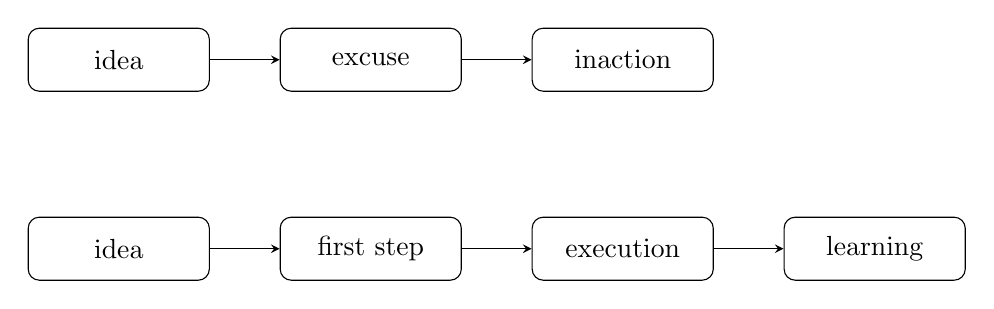
\begin{tikzpicture}[>=stealth]
\node[draw, rounded corners, minimum width=2.3cm, minimum height=0.8cm] (a1) at (0,1.2) {idea};
\node[draw, rounded corners, minimum width=2.3cm, minimum height=0.8cm] (a2) at (3.2,1.2) {excuse};
\node[draw, rounded corners, minimum width=2.3cm, minimum height=0.8cm] (a3) at (6.4,1.2) {inaction};

\node[draw, rounded corners, minimum width=2.3cm, minimum height=0.8cm] (b1) at (0,-1.2) {idea};
\node[draw, rounded corners, minimum width=2.3cm, minimum height=0.8cm] (b2) at (3.2,-1.2) {first step};
\node[draw, rounded corners, minimum width=2.3cm, minimum height=0.8cm] (b3) at (6.4,-1.2) {execution};
\node[draw, rounded corners, minimum width=2.3cm, minimum height=0.8cm] (b4) at (9.6,-1.2) {learning};

\draw[->] (a1) -- (a2);
\draw[->] (a2) -- (a3);

\draw[->] (b1) -- (b2);
\draw[->] (b2) -- (b3);
\draw[->] (b3) -- (b4);
\end{tikzpicture}
\end{figure}

The inserted sponsor material should be read structurally rather than analytically. Its role in the lecture is to reduce the distance between idea and first step. In that sense it is consistent with the chapter's broader theme: execution does not require infinite readiness; it requires crossing the threshold from intention to action.

\section{High Income, Restraint, and Generational Choice}

The Jameis Winston interview reopens the chapter from a different direction. Here the wealth engine is not a business sale but elite income. Nevertheless the structure remains recognizably the same. The lecture wants to know not merely how much money came in, but how that money was partitioned and protected.

The first ledger is straightforward:
\begin{align}
Y_{\text{Jameis,max}}&\approx \$25\times 10^6,\\
C_{\text{spend}}&\approx C_{\text{endorsements}},\\
C_{\text{game}}&\text{ retained rather than used for current life.}
\end{align}

This is a disciplined partition rule. The lecture does not formalize it as a budget equation, but the logic is plain enough: if current spending is carried by endorsements, then the primary athletic income is given time to persist.

The second ledger concerns duration:
\begin{equation}
T_{\text{NFL}}=11\,\mathrm{yr},\qquad
T_{\text{NFL,avg}}\in[2,3]\,\mathrm{yr}.
\end{equation}
The speaker attributes this longevity to gratitude, hard work, and never giving up. We should preserve that sequence in prose rather than forcing it into a false theorem. The lecture is careful here. It lets gratitude function as a stabilizing posture before it lets it function as an explanation.

\subsection{Question \& Answer}

How does a rich family begin if one did not come from one?

The answer given in the lecture is simple and severe: through choices. The host says that a rich family is going to come from the player. The player corrects the phrase: a wealthy family will come from him, through the choices and decisions that are made. This is the right correction. Wealth here is not treated as a spectacular one-time event. It is treated as an intergenerational consequence of restraint, duration, and allocation.

Faith is part of the same structure. The lecture does not present faith as a cash-flow identity. It presents it as the prior order that lets endurance remain stable under pressure. One begins with God, then education, then the conviction that one can do what one sets one's mind to. In the football version of the rule, one simply never gives up. The economic effect is indirect but important: a stable interior order can protect a large income from turning into a large ruin.

\section{Leverage, Collapse, and the Person Left Standing}

The Adam Weitzman interview closes the chapter by making the arithmetic morally harder. We begin again with scale,
\begin{align}
Y_{\text{metal,max}}&\in[\$60,\$70]\times 10^6,\\
V_{\text{firm}}&\approx \$10^9,\\
n_{\text{negotiation}}&=7.5/10,
\end{align}
but the lecture refuses to stop there. It turns quickly to leverage, ego, arrest, prison, rebuilding, sacrifice, and finally happiness.

The capital-structure story here is explicitly different from the earlier logistics operator's story. Early growth was financed with loans. The speaker says he was overleveraged. It was bad. He later paid those loans off, and he still says leverage is part of growth. But the mature lesson is different from the youthful method: the leverage days are over. This is not a contradiction. It is the lecture's most explicit reminder that a tactic which helps expansion can later become a source of fragility.

The personal collapse is also timed:
\begin{equation}
T_{\text{prison}}=1\,\mathrm{yr},\qquad
T_{\text{pre-prison flux}}\approx 4\,\mathrm{yr}.
\end{equation}
The lecture is careful to note that prison is not only the sentence. It is also the long interval between arrest and confinement, the period in which uncertainty itself becomes punishment.

What follows is not legal theory but a rule of character. Nobody is coming to save you. There is no money tree in the backyard. Stay focused. Sacrifice. Do not put yourself in positions where you must make the bad choice you already recognize as bad. Read the small print. If you guarantee something, you are liable. These are not elegant abstractions, but they are consistent with the rest of the lecture: the path to durable wealth is full of interfaces where fantasy must yield to exact structure.

The final correction is psychological. One should not believe one's own propaganda. Money is called a mirage. The speaker says his greatest strength is that he can be happy with nothing. This is where the chapter closes the circle. At the beginning, wealth appeared as spectacle. At the end, it is subordinated to the character that remains after spectacle, collapse, and recovery have all passed through the same life.

\section{Summary}

The lecture teaches by ordered contrast. First it shows us scale. Then it shows us how hard it is to reach the people who embody that scale. Then it extracts mechanisms. Those mechanisms are not uniform, but they rhyme:

\begin{itemize}
\item A founder-built company becomes more saleable as founder dependence falls.
\item Rough operating work can be converted into land, tenants, and generational holdings.
\item Debt can enlarge scale, but resilience depends on how much room remains after error.
\item High income becomes durable wealth only when spending is partitioned and restrained.
\item Ideas become valuable only after the first step has been taken.
\end{itemize}

What makes this lecture stronger than a mere catalog of rich people is that it does not leave wealth at the level of numbers. It continually asks what sort of structure, and finally what sort of person, can carry money without being destroyed by it.